%%
% Please see https://bitbucket.org/rivanvx/beamer/wiki/Home for obtaining beamer.
%%
\documentclass[handout]{beamer}
%\usetheme{Warsaw}

\usepackage{blkarray}
\usepackage{bigstrut}
\usepackage{amsmath}
\usepackage{bbm}
\usepackage{harpoon}
\usepackage{caption}
\usepackage{subcaption}
\usefonttheme[onlymath]{serif}

\makeatletter
\let\BA@quicktrue\BA@quickfalse
\makeatother

\renewcommand{\vec}[1]{ {\bf #1} }
\newcommand{\mat}[1]{ \vec{#1} }
\newcommand{\abs}[1]{ \left\lvert #1 \right\rvert }

\title{A Supervised Learning Approach to Predicting Multigrid Convergence}
\author[N. Nytko]{Nicolas Nytko\\[3mm]Matthew West, Luke Olson, Scott MacLachlan}
\date{\today}

\begin{document}
\frame{\titlepage}


% Overview
\begin{frame}
  \frametitle{Introduction}
  todo: insert introduction
\end{frame}


% Poisson intro
\begin{frame}
  \frametitle{Poisson Problem}
  \begin{itemize}
  \item Look at the 1D variable coefficients case w/ homogeneous Dirichlet conditions
    \[ -\nabla \cdot \left(k\left(\vec{x}\right) \nabla \vec{y} \right) = f \]
    \[ \Omega = \left[-1, 1\right] \quad \partial\Omega = 0 \]
  \item Discretized on $N=31$ internal points using finite differences, $k\left(\vec{x}\right)$ is discretized on midpoints to preserve symmetry.
  \item For arbitrary C/F splitting, can we predict convergence rate and optimal relaxation weight?
  \end{itemize}
\end{frame}


\begin{frame}
  \frametitle{Training Dataset}
  \begin{itemize}
  \item For ``traditional'' machine learning we need a dataset.
    \pause
  \item Idea: Run a \textit{whole lot} of multigrid iterations.
    \pause
  \item Run multigrid iterations and record convergence rate and relaxation weight for randomly generated C/F splittings and problem setups.
  \end{itemize}
  \begin{center}
    \includegraphics[width=0.8\textwidth]{figures/multigrid.png}
  \end{center}
\end{frame}


\begin{frame}
  \frametitle{Dataset Generation}
  \begin{itemize}
  \item Start from ``reference'' splittings, which are evenly spaced coarse points on a grid.
  \item Randomly perturb each reference in several trials, according to \[ p = \left\{ 0.01 \quad 0.05 \quad 0.1 \quad 0.25 \quad 0.5 \quad 0.75 \right\}. \]
  \item Generate variable coefficients such that \[ k\left(\vec{x}\right) = \begin{cases}
\alpha \\
\text{rand()}\left(\alpha + 1\right) \\
\alpha\cos\left(\pi x \beta\right) + \gamma \\
\abs{\sum_{i=1}^5 \alpha_i x^i} + 0.01
\end{cases}. \]
  \end{itemize}
\end{frame}


\begin{frame}
  \frametitle{Convolutional Network}
  \begin{itemize}
  \item Take the C/F splittings, run in multigrid solver to find convergence rate and relaxation weight that maximizes the former.
  \item Use the data to train a \textit{1D convolutional network} that predicts convergence, Jacobi relaxation.
  \end{itemize}

  \begin{table}[t]
\centering
\begin{tabular}{|l|l|l|l|}
\hline
Model & Dataset & Value \\

\hline
Jacobi Weight & Training & $1.8331 \times 10^{-3}$ \\
Jacobi Weight &  Testing & $1.8396 \times 10^{-3}$ \\
\hline
Convergence Factor & Training & $1.4839 \times 10^{-3}$ \\
Convergence Factor & Testing & $1.5171 \times 10^{-3}$ \\
\hline
\end{tabular}
\caption{Mean squared error (MSE) between predicted and true Jacobi weight, convergence factor.}
\label{tab:poisson_loss}
\end{table}
\end{frame}


\begin{frame}
  \frametitle{CNN Performance}
  \begin{figure}[h]
  \centering
  \begin{subfigure}{.48\textwidth}
    \includegraphics[width=\textwidth]{figures/poisson_conv_test_pred.png}
    \caption{Testing predictions}
  \end{subfigure}
  \begin{subfigure}{.48\textwidth}
    \includegraphics[width=\textwidth]{figures/poisson_jacobi_test_pred.png}
    \caption{Training predictions}
  \end{subfigure}
  \caption{(a) Predicted convergence values vs. true convergence values, (b) Predicted relaxation weights vs true relaxation weights.  Values closer to the diagonal represent more accurate predictions. }
  \label{fig:poisson_conv_pred}
\end{figure}
\end{frame}


\begin{frame}
  What we learned: \pause Poisson is too easy!
  \newline\newline
  \pause

  Let's try learning a more difficult problem.
\end{frame}


\begin{frame}
  \frametitle{Convection-Diffusion Problem}
  Try out a specific convection-diffusion problem,
  \[\vec{w}\cdot\nabla u -k\nabla^2u = f,\]
  on 2D square, $\Omega = \left[-1,1\right]^2$, discretized as quadrilateral finite elements.  Use  $k=0.1$, $\vec{w} = \begin{bmatrix} 2y(1-x^2) & 2x(1-y^2)  \end{bmatrix}$.  Apply Dirichlet conditions as one ``hot'' wall and three ``cold'' walls.
  \begin{figure}[h]
    \includegraphics[width=0.4\textwidth]{figures/recirculating.png}
  \end{figure}
\end{frame}


\begin{frame}
  \frametitle{Dataset Generation, Convection-Diffusion}
  \begin{itemize}
  \item Discretize on a $25 \times 25$ structured grid.
  \item Start from ``reference'' splittings, all fine, all coarse, AMG output, etc.
  \item Randomly perturb each reference in several trials, according to \[ p = \left\{ 0.01 \quad 0.05 \quad 0.1 \quad 0.25 \quad 0.5 \quad 0.75 \right\}. \]
  \item Don't generate coefficient values for now.
  \item Take output and run through 50 iteration multigrid solver to find convergence rate.
  \end{itemize}
\end{frame}


\begin{frame}
  \frametitle{Convection-Diffusion Convolution}
  \begin{itemize}
    \item 2D structured grid $\Rightarrow$ train 2D convolutional network to predict convergence.
  \end{itemize}
  \begin{figure}[h]
  \centering
  \begin{subfigure}{.48\textwidth}
    \includegraphics[width=\textwidth]{figures/poisson_conv_test_pred.png}
    \caption{Testing predictions}
    \label{subfig:poisson_conv_test}
  \end{subfigure}
  \begin{subfigure}{.48\textwidth}
    \includegraphics[width=\textwidth]{figures/poisson_conv_train_pred.png}
    \caption{Training predictions}
    \label{subfig:poisson_conv_train}
  \end{subfigure}
  \caption{Predicted convergence values vs. true convergence values on (\ref{subfig:poisson_conv_test}) testing and (\ref{subfig:poisson_conv_train}) training datasets for Poisson equation. Values closer to the diagonal represent more accurate predictions. }
  \label{fig:poisson_conv_pred}
\end{figure}
\end{frame}


\begin{frame}
  \frametitle{CNN to GNN}
  \begin{itemize}
  \item Classical convolution techniques work okay on structured, grid-like inputs.
  \item Very restrictive in terms of mesh data we can use for FEM solvers.
  \item Take a look at some network architectures that allow for unstructured data: introduce \textit{graph-nets}.
  \end{itemize}
\end{frame}


\begin{frame}
  \frametitle{Graphnets Motivation}
  Take FEM matrix, convert to graph and try to learn properties about the system.
  \begin{figure}[h]
  \begin{subfigure}{.40\textwidth}
    \includegraphics[width=\textwidth]{figures/sparse.png}
  \end{subfigure}
  \begin{subfigure}{.08\textwidth}
    \[ \Longrightarrow \]
  \end{subfigure}
  \begin{subfigure}{.40\textwidth}
    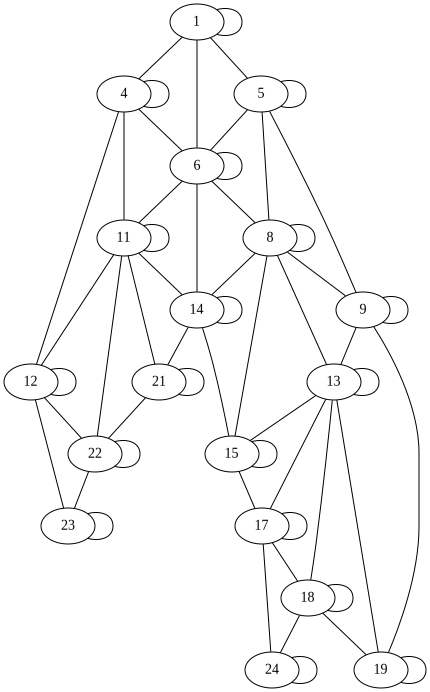
\includegraphics[width=0.7\textwidth]{figures/graph.png}
  \end{subfigure}
\end{figure}
\end{frame}


\begin{frame}
  \frametitle{Message-Passing Graph Convolutions}
  \begin{itemize}
  \item Many graph convolution implementations, one such is the \textit{Message-Passing Graph} layer.
  \item Nodes learn optimal ``messages'' to pass via edges.  Each node passes this message to other nodes in its neighborhood.
  \item Update given by:
  \begin{equation*}\label{eqn:mpnn_prop}
    \left(\mat{H}^{(i)}\right)_j = \frac{1}{\abs{\mathcal{N}\left(j\right)}} \sum_{k\in\mathcal{N}\left(j\right)} F^{(i)}\left(e_{j,k}\right)\left(\mat{H}^{(i-1)}\right)_k + \vec{b}^{(i)}
  \end{equation*}
  \item Stacking multiple of these layers approximates traditional grid-based convolution.
  \end{itemize}
\end{frame}


\begin{frame}
  \frametitle{Message-Passing Architecture}
  \begin{itemize}
  \item Pass node C/F values, $\mat{X}$, through 4 MPN layers to get $\mat{H}^{(i)}, \enskip i\in\left\{1,2,3,4\right\}$.
  \item Stack historical values to both simulate residual-style networks and give more information to aggregator:
    \[ \mat{R} =
\begin{bmatrix}
\hdots & \mat{X}^T & \hdots \\
\hdots & \left(\mat{H}^{(1)}\right)^T & \hdots \\
\hdots & \left(\mat{H}^{(2)}\right)^T & \hdots \\
\hdots & \left(\mat{H}^{(3)}\right)^T & \hdots \\
\hdots & \left(\mat{H}^{(4)}\right)^T & \hdots \\
\end{bmatrix} \]
\item Run each set of nodal values through linear NN, take average for final convergence rate:
  \[ y=\frac{1}{N} \sum_j \sigma\left( \left( \vec{r}_j \mat{W}^{(5)} + \vec{b}^{(5)} \right)\mat{W}^{(6)} + \vec{b}^{(6)} \right) \]
  \end{itemize}
\end{frame}


\begin{frame}
  \frametitle{Message-Passing Dataset}
  \begin{itemize}
  \item Decoupled the neural network from a fixed input size due to final aggregation step.
  \item Can have variable-sized input.  Now generate and train on  a variably-sized dataset of four mesh sizes:
  \[ \left\{ 15\times 15 \quad 25\times 25 \quad 35\times 35 \quad 50 \times 50 \right\} \]
  \end{itemize}
\end{frame}


\begin{frame}
  \frametitle{Message-Passing Performance}
  \begin{figure}[h]
  \centering
  \begin{subfigure}{.48\textwidth}
    \includegraphics[width=\textwidth]{figures/cd_var_conv_mpnn_test_pred.png}
    \caption{Testing predictions}
    \label{subfig:cd_mpnn_test}
  \end{subfigure}
  \begin{subfigure}{.48\textwidth}
    \includegraphics[width=\textwidth]{figures/cd_var_conv_mpnn_train_pred.png}
    \caption{Training predictions}
    \label{subfig:cd_mpnn_train}
  \end{subfigure}
  \caption{Predicted convergence rates vs. true convergence rates on (\ref{subfig:cd_mpnn_test}) testing and (\ref{subfig:cd_mpnn_train}) training datasets for model convection-diffusion problem, using an Edge-Conditioned Convolution network. Values closer to the diagonal represent more accurate predictions.}
  \label{fig:cd_mpnn_pred}
\end{figure}
\end{frame}


%% \begin{frame}
%%   ??? put something here ???

%%   this seems short-ish so far
%% \end{frame}


\begin{frame}
  \frametitle{Future Directions}
  \begin{itemize}
  \item Try out some more interesting problems:
  \begin{figure}[h]
  \centering
  \begin{subfigure}{.70\textwidth}
    \includegraphics[width=\textwidth]{figures/cd_bfs.png}
  \end{subfigure}
  \begin{subfigure}{.70\textwidth}
    \includegraphics[width=\textwidth]{figures/cd_cyl.png}
  \end{subfigure}
  \end{figure}
  \item Pick between different AMG methods with predictions.
  \item Use predictions in an optimization routine to find most convergent C/F splitting.
  \end{itemize}
\end{frame}

\end{document}
